\documentclass[12pt]{article}
\usepackage[margin=1in]{geometry}

% Font and Language (Computer Modern, xelatex)
\usepackage{polyglossia}
\setmainlanguage{greek}
\setotherlanguage{english}
\newfontfamily\greekfont{FreeSerif}
\newfontfamily\greekfonttt{FreeSerif}

% Math
\usepackage{amsmath}

% General
\usepackage{graphicx}
\graphicspath{ {./} }
\usepackage{caption}
\captionsetup{labelsep=none, font={small,it}}
\renewcommand{\thefigure}{}
\usepackage{float}
\usepackage{ragged2e}
\usepackage{fancyhdr}
\usepackage{titlesec}
\usepackage[table]{xcolor}
\usepackage{hyperref}
\usepackage{listings}
\arrayrulecolor{black}

% Listings configuration with colors and frame
\lstset{
    backgroundcolor=\color{white},
    frame=single,
    framesep=4pt,
    framerule=0.5pt,
    rulecolor=\color{gray!50},
    basicstyle=\ttfamily\small,
    keywordstyle=\color{blue}\bfseries,
    stringstyle=\color{red},
    commentstyle=\color{green!50!black},
    numberstyle=\tiny\color{gray},
    numbers=left,
    numbersep=5pt,
    stepnumber=1,
    showstringspaces=false,
    tabsize=4,
    breaklines=true,
    breakatwhitespace=false,
    language=VHDL
}
\hypersetup{
    colorlinks=true,
    linkcolor=blue
}

% Layout
\setlength{\parindent}{0pt}
\setlength{\parskip}{0.5em}

% Title
\title{}
\author{}
\date{}


\begin{document}
    \begin{titlepage}
        \begin{center}

            \begin{minipage}{0.3\textwidth}
                
\includegraphics[width=\linewidth]{../../ntua_logo.png}
            \end{minipage}
            \hfill
            \begin{minipage}{0.65\textwidth}
                \centering
                {\LARGE \textbf{Εθνικό Μετσόβιο Πολυτεχνείο}}\\[0.3cm]
                {\large \textbf{Σχολή Ηλεκτρολόγων Μηχανικών \& Μηχανικών Υπολογιστών}}\\[0.2cm]
                \rule{\linewidth}{0.5pt}\\[0.3cm]
                {\large Εξάμηνο 8\textsuperscript{o}}\\
                {\large \textbf{Ψηφιακά Συστήματα VLSI}}\\
            \end{minipage}

            \vspace{2cm}

            {\Huge \textbf{3η Εργαστηριακή Άσκηση}}\\[1cm]

            {\Large \textbf{Υλοποίηση FIR Φίλτρου}}\\[5cm]

            {\Large \textbf{Μέλη Ομάδας}}\\[0.5cm]

            \begin{tabular}{rl}
                \textbf{Καβαδάκης Σωτήρης} & 03122035 \\
                \textbf{Κοντοπίδης Δημήτρης} & 03122025 \\
            \end{tabular}

            \vfill

            {\large Αθήνα, Μάρτιος 2026}

        \end{center}
    \end{titlepage}
    \clearpage

% ==============================================================================
% SECTION 1: Αρχιτεκτονική FIR Φίλτρου
% ==============================================================================
\section*{Αρχιτεκτονική 8-tap FIR Φίλτρου}

Το FIR φίλτρο υλοποιεί την εξίσωση:
\[
    y[n] = \sum_{k=0}^{7} h[k]\, x[n-k]
    = h[0]\,x[n] + h[1]\,x[n-1] + \ldots + h[7]\,x[n-7]
\]

για $N = 8$ bits εύρος δεδομένων εισόδου $x$ (unsigned) και σταθερούς συντελεστές $h[k]$ επίσης 8-bit unsigned.

Η κορυφαία οντότητα \texttt{FIR} έχει δομική (Structural) αρχιτεκτονική και αποτελείται από τέσσερις υπο-μονάδες:

\begin{itemize}
    \item \textbf{MAC} (Multiply-Accumulate Unit): υπολογίζει το $y[n]$ συσσωρεύοντας τα γινόμενα $h[k] \cdot x[n-k]$.
    \item \textbf{ROM}: αποθηκεύει τους σταθερούς συντελεστές $h[0]\ldots h[7]$.
    \item \textbf{RAM}: υλοποιεί sliding window των τελευταίων 8 τιμών εισόδου $x[n]\ldots x[n-7]$.
    \item \textbf{Control Unit}: παράγει τις διευθύνσεις ROM/RAM, το σήμα \texttt{mac\_init} και τα σήματα \texttt{valid\_out}/\texttt{we}.
\end{itemize}

\subsection*{Σήματα Εισόδου/Εξόδου}

\begin{itemize}
    \item \texttt{i\_clk}: Σήμα ρολογιού
    \item \texttt{i\_rst}: Ασύγχρονο reset (ενεργό στο '1')
    \item \texttt{i\_valid\_in}: Εγκυρότητα νέας εισόδου $x$
    \item \texttt{i\_x(7:0)}: Τιμή εισόδου $x[n]$ (8-bit unsigned)
    \item \texttt{o\_valid\_out}: Εγκυρότητα εξόδου $y$
    \item \texttt{o\_y(18:0)}: Τιμή εξόδου $y[n]$ (19-bit)
\end{itemize}

Το εύρος εξόδου $L = 19$ bits προκύπτει από την ανάγκη αναπαράστασης χωρίς υπερχείλιση: κάθε γινόμενο $h[k] \cdot x[n-k]$ δύο 8-bit αριθμών απαιτεί 16 bits, και η άθροιση 8 τέτοιων γινομένων απαιτεί επιπλέον $\lceil\log_2 8\rceil = 3$ bits, άρα συνολικά $16 + 3 = 19$ bits.

\subsection*{Λειτουργία}

\begin{enumerate}
    \item Κάθε φορά που το \texttt{valid\_in} είναι ενεργό, η τιμή $x[n]$ αποθηκεύεται στη θέση 0 της RAM, ενώ οι ήδη αποθηκευμένες τιμές ολισθαίνουν κατά μία θέση (sliding window).
    \item Η Control Unit ξεκινά έναν μετρητή 0--7 που διευθυνσιοδοτεί ταυτόχρονα ROM και RAM.
    \item Σε κάθε από τους 8 κύκλους, η MAC συσσωρεύει το γινόμενο $h[k] \cdot x[n-k]$.
    \item Μετά τον 8ο κύκλο, το \texttt{valid\_out} ενεργοποιείται και η έξοδος $y[n]$ είναι έγκυρη.
\end{enumerate}

Το φίλτρο δέχεται νέα είσοδο κάθε 8 κύκλους ρολογιού και παράγει αντίστοιχα μία νέα έγκυρη έξοδο κάθε 8 κύκλους.

% ------------------------------------------------------------------------------
\subsection*{Κώδικας VHDL -- Top-level \texttt{FIR}}
% ------------------------------------------------------------------------------

\begin{lstlisting}[language=VHDL]
library IEEE;
use IEEE.STD_LOGIC_1164.ALL;
use IEEE.STD_LOGIC_UNSIGNED.ALL;

entity FIR is
    port (
        i_clk       : in  std_logic;
        i_rst       : in  std_logic;
        i_valid_in  : in  std_logic;
        i_x         : in  std_logic_vector(7 downto 0);
        o_valid_out : out std_logic;
        o_y         : out std_logic_vector(18 downto 0)
    );
end FIR;

architecture Structural of FIR is

    signal rom_address_sig : std_logic_vector(2 downto 0);
    signal ram_address_sig : std_logic_vector(2 downto 0);
    signal mac_init_sig    : std_logic;
    signal rom_out_sig     : std_logic_vector(7 downto 0);
    signal ram_out_sig     : std_logic_vector(7 downto 0);
    signal ram_we_sig      : std_logic;

begin

    ControlUnit: entity work.control_unit
        port map (
            i_clk         => i_clk,
            i_rst         => i_rst,
            i_valid_in    => i_valid_in,
            o_mac_init    => mac_init_sig,
            o_rom_address => rom_address_sig,
            o_ram_address => ram_address_sig,
            o_valid_out   => o_valid_out,
            o_we          => ram_we_sig
        );

    ROM: entity work.mlab_rom
        port map (
            i_clk     => i_clk,
            i_en      => '1',
            i_addr    => rom_address_sig,
            o_rom_out => rom_out_sig
        );

    RAM: entity work.mlab_ram
        port map (
            i_clk  => i_clk,
            i_en   => '1',
            i_rst  => i_rst,
            i_we   => ram_we_sig,
            i_addr => ram_address_sig,
            i_di   => i_x,
            o_do   => ram_out_sig
        );

    MAC: entity work.mac
        port map (
            i_clk      => i_clk,
            i_mac_init => mac_init_sig,
            i_rom_data => rom_out_sig,
            i_ram_data => ram_out_sig,
            o_y        => o_y
        );

end Structural;
\end{lstlisting}

% ==============================================================================
% SECTION 2: Υπο-μονάδες
% ==============================================================================
\newpage
\section*{Περιγραφή Υπο-μονάδων}

% ------------------------------------------------------------------------------
\subsection*{1. MAC -- Μονάδα Πολλαπλασιασμού με Συσσώρευση}
% ------------------------------------------------------------------------------

Η MAC υλοποιεί τη λειτουργία:
\[
    a \leftarrow a + b \times c
\]

όπου $b = \texttt{rom\_out}$ (συντελεστής $h[k]$), $c = \texttt{ram\_out}$ (δείγμα $x[n-k]$), και $a$ ο συσσωρευτής.

Η μονάδα ελέγχεται από το σήμα \texttt{mac\_init}: όταν είναι ενεργό, ο συσσωρευτής αρχικοποιείται με το πρώτο γινόμενο ($h[0] \cdot x[n]$) αντί να προσθέσει στην προηγούμενη τιμή. Αυτό διασφαλίζει ότι κάθε νέος υπολογισμός $y[n]$ ξεκινά από μηδέν.

Η υλοποίηση είναι behavioral με χρήση της βιβλιοθήκης \texttt{std\_logic\_unsigned}.

\begin{lstlisting}[language=VHDL]
library IEEE;
use IEEE.STD_LOGIC_1164.ALL;
use IEEE.STD_LOGIC_UNSIGNED.ALL;
use IEEE.math_real.all;

entity mac is
    port (
        i_clk      : in  std_logic;
        i_rom_data : in  std_logic_vector(7 downto 0);
        i_ram_data : in  std_logic_vector(7 downto 0);
        i_mac_init : in  std_logic;
        o_y        : out std_logic_vector(18 downto 0)
    );
end mac;

architecture Behavioral of mac is
    signal acc : std_logic_vector(18 downto 0) := (others => '0');
begin
    process(i_clk)
    begin
        if rising_edge(i_clk) then
            if i_mac_init = '1' then
                acc         <= (others => '0');
                acc(15 downto 0) <= i_ram_data * i_rom_data;
            else
                acc <= acc + i_ram_data * i_rom_data;
            end if;
        end if;
    end process;
    o_y <= acc;
end Behavioral;
\end{lstlisting}

% ------------------------------------------------------------------------------
\subsection*{2. ROM -- Μνήμη Συντελεστών}
% ------------------------------------------------------------------------------

Η ROM αποθηκεύει τους 8 σταθερούς συντελεστές του φίλτρου. Υλοποιείται ως synchronous read-only memory (registered output, μία καθυστέρηση κύκλου). Οι συντελεστές είναι:

\begin{table}[H]
    \centering
    \begin{tabular}{|c|c|c|c|c|c|c|c|c|}
        \hline
        \textbf{Διεύθυνση} & 0 & 1 & 2 & 3 & 4 & 5 & 6 & 7 \\
        \hline
        \textbf{h[k]} & 8 & 7 & 6 & 5 & 4 & 3 & 2 & 1 \\
        \hline
    \end{tabular}
    \caption{Συντελεστές ROM}
\end{table}

\begin{lstlisting}[language=VHDL]
library IEEE;
use IEEE.STD_LOGIC_1164.ALL;
use ieee.std_logic_unsigned.all;

entity mlab_rom is
    generic (
        coeff_width : integer := 8
    );
    Port (
        i_clk     : in  STD_LOGIC;
        i_en      : in  STD_LOGIC;
        i_addr    : in  STD_LOGIC_VECTOR(2 downto 0);
        o_rom_out : out STD_LOGIC_VECTOR(coeff_width-1 downto 0)
    );
end mlab_rom;

architecture Behavioral of mlab_rom is
    type rom_type is array (7 downto 0)
        of std_logic_vector(coeff_width-1 downto 0);
    signal rom : rom_type := (
        "00001000", "00000111", "00000110", "00000101",
        "00000100", "00000011", "00000010", "00000001");
    signal rdata : std_logic_vector(coeff_width-1 downto 0)
        := (others => '0');
begin
    rdata <= rom(conv_integer(i_addr));
    process(i_clk)
    begin
        if rising_edge(i_clk) then
            if i_en = '1' then
                o_rom_out <= rdata;
            end if;
        end if;
    end process;
end Behavioral;
\end{lstlisting}

% ------------------------------------------------------------------------------
\subsection*{3. RAM -- Sliding Window Μνήμη Εισόδου}
% ------------------------------------------------------------------------------

Η RAM αποθηκεύει τις 8 πιο πρόσφατες τιμές εισόδου $x[n], x[n-1], \ldots, x[n-7]$. Υλοποιείται ως \textbf{write-first} μνήμη: κατά την εγγραφή, τα νέα δεδομένα εμφανίζονται αμέσως και στην έξοδο στον ίδιο κύκλο.

Κατά τη λειτουργία εγγραφής (\texttt{we='1'}):
\begin{itemize}
    \item Τα περιεχόμενα ολισθαίνουν: $\text{RAM}[7:1] \leftarrow \text{RAM}[6:0]$
    \item Η νέα τιμή $x[n]$ αποθηκεύεται στη θέση 0: $\text{RAM}[0] \leftarrow x[n]$
\end{itemize}

Κατά reset, όλες οι θέσεις αρχικοποιούνται στο '0'. Αρχικά, πριν φτάσουν 8 τιμές, οι άδειες θέσεις της RAM θεωρούνται μηδέν.

\begin{lstlisting}[language=VHDL]
library ieee;
use ieee.std_logic_1164.all;
use ieee.std_logic_unsigned.all;

entity mlab_ram is
    generic (
        data_width : integer := 8
    );
    port (
        i_clk  : in  std_logic;
        i_we   : in  std_logic;
        i_en   : in  std_logic;
        i_rst  : in  std_logic;
        i_addr : in  std_logic_vector(2 downto 0);
        i_di   : in  std_logic_vector(data_width-1 downto 0);
        o_do   : out std_logic_vector(data_width-1 downto 0)
    );
end mlab_ram;

architecture Behavioral of mlab_ram is
    type ram_type is array (7 downto 0)
        of std_logic_vector(data_width-1 downto 0);
    signal RAM : ram_type := (others => (others => '0'));
begin
    process(i_clk, i_rst)
    begin
        if i_rst = '1' then
            RAM <= (others => (others => '0'));
        elsif rising_edge(i_clk) then
            if i_en = '1' then
                if i_we = '1' then
                    RAM(7 downto 1) <= RAM(6 downto 0); -- shift
                    RAM(0) <= i_di;
                    o_do   <= i_di;                     -- write-first
                else
                    o_do <= RAM(conv_integer(i_addr));
                end if;
            end if;
        end if;
    end process;
end Behavioral;
\end{lstlisting}

% ------------------------------------------------------------------------------
\subsection*{4. Control Unit -- Μονάδα Ελέγχου}
% ------------------------------------------------------------------------------

Η Control Unit διαχειρίζεται την αλληλουχία λειτουργίας του φίλτρου μέσω ενός 4-bit μετρητή. Οι καταστάσεις λειτουργίας είναι:

\begin{itemize}
    \item \textbf{IDLE} (\texttt{counter = "1000"}): Αναμονή. Μόλις το \texttt{valid\_in} γίνει '1', γράφεται το $x[n]$ στη RAM (\texttt{we='1'}), τίθεται σε pipeline ο \texttt{mac\_init} και ο μετρητής μηδενίζεται.
    \item \textbf{ACTIVE} (\texttt{counter = 0..7}): Σε κάθε κύκλο, ο μετρητής αυξάνεται κατά 1 και δίνει την επόμενη διεύθυνση ROM/RAM. Οι διευθύνσεις ROM και RAM είναι πάντα ταυτόσημες (\texttt{counter[2:0]}). Στον τελευταίο κύκλο (\texttt{counter = "0111"}), τίθεται σε pipeline το \texttt{valid\_out}. Αν έχει φτάσει νέα είσοδος, γίνεται straight loop-back στο 0 χωρίς επιστροφή στο IDLE.
\end{itemize}

Η χρήση pipeline registers (\texttt{mac\_init\_next}, \texttt{valid\_out\_next}) αντισταθμίζει την καθυστέρηση ενός κύκλου της ROM (registered output), εξασφαλίζοντας ότι το \texttt{mac\_init} και το \texttt{valid\_out} εμφανίζονται στη σωστή χρονική στιγμή.

\begin{lstlisting}[language=VHDL]
library IEEE;
use IEEE.STD_LOGIC_1164.ALL;
use IEEE.STD_LOGIC_UNSIGNED.ALL;

entity control_unit is
    port (
        i_clk         : in  std_logic;
        i_rst         : in  std_logic;
        i_valid_in    : in  std_logic;
        o_rom_address : out std_logic_vector(2 downto 0);
        o_ram_address : out std_logic_vector(2 downto 0);
        o_mac_init    : out std_logic;
        o_we          : out std_logic;
        o_valid_out   : out std_logic
    );
end control_unit;

architecture Behavioral of control_unit is
    signal counter        : std_logic_vector(3 downto 0) := "1000";
    signal mac_init_next  : std_logic := '0';
    signal valid_out_next : std_logic := '0';
begin
    o_rom_address <= counter(2 downto 0);
    o_ram_address <= counter(2 downto 0);

    process(i_clk, i_rst)
    begin
        if i_rst = '1' then
            counter        <= "1000";
            o_mac_init     <= '0';
            o_we           <= '0';
            o_valid_out    <= '0';
            mac_init_next  <= '0';
            valid_out_next <= '0';
        elsif rising_edge(i_clk) then
            o_mac_init  <= mac_init_next;
            o_valid_out <= valid_out_next;

            o_we           <= '0';
            mac_init_next  <= '0';
            valid_out_next <= '0';

            if counter = "1000" then           -- IDLE
                if i_valid_in = '1' then
                    o_we          <= '1';
                    mac_init_next <= '1';
                    counter       <= "0000";
                end if;
            else                               -- ACTIVE
                if counter = "0111" then
                    valid_out_next <= '1';
                    if i_valid_in = '1' then
                        o_we          <= '1';
                        mac_init_next <= '1';
                        counter       <= "0000";
                    else
                        counter       <= "1000";
                    end if;
                else
                    counter <= counter + 1;
                end if;
            end if;
        end if;
    end process;
end Behavioral;
\end{lstlisting}

% ==============================================================================
% SECTION 3: Testbench
% ==============================================================================
\newpage
\section*{Testbench}

Υλοποιήθηκαν δύο testbenches για τον έλεγχο της ορθής λειτουργίας του φίλτρου.

% ------------------------------------------------------------------------------
\subsection*{1. Testbench Εργαστηρίου (\texttt{fir\_tb\_lab.vhd})}
% ------------------------------------------------------------------------------

Το testbench αυτό ελέγχει τη λειτουργία του φίλτρου με μια σειρά από 20 πραγματικές εισόδους. Στέλνει το κάθε $x[n]$ με διάστημα 8 κύκλων και παρακολουθεί οπτικά (μέσω waveform) τα \texttt{valid\_out} και $y$. Περιλαμβάνει:

\begin{itemize}
    \item Αρχικό reset 2 κύκλων.
    \item Αποστολή 20 τιμών εισόδου (π.χ. \texttt{0xD0}, \texttt{0xE7}, \texttt{0x20}, \ldots) με χρήση \texttt{valid\_in='1'} για 1 κύκλο και αναμονή 7 κύκλων μεταξύ τους.
\end{itemize}

\begin{lstlisting}[language=VHDL]
library IEEE;
use IEEE.STD_LOGIC_1164.ALL;
use IEEE.STD_LOGIC_UNSIGNED.ALL;

entity tb_FIR is
end tb_FIR;

architecture Behavioral of tb_FIR is

    constant N          : integer := 8;
    constant L          : integer := 19;
    constant CLK_PERIOD : time    := 10 ns;

    signal tb_clk       : std_logic := '0';
    signal tb_rst       : std_logic := '0';
    signal tb_valid_in  : std_logic := '0';
    signal tb_x         : std_logic_vector(N-1 downto 0) := (others => '0');
    signal tb_valid_out : std_logic;
    signal tb_y         : std_logic_vector(L-1 downto 0);

begin

    UUT: entity work.FIR
        port map (
            i_clk       => tb_clk,
            i_rst       => tb_rst,
            i_valid_in  => tb_valid_in,
            i_x         => tb_x,
            o_valid_out => tb_valid_out,
            o_y         => tb_y
        );

    clk_process: process
    begin
        tb_clk <= '0'; wait for CLK_PERIOD / 2;
        tb_clk <= '1'; wait for CLK_PERIOD / 2;
    end process;

    stim_process: process
    begin
        tb_rst <= '1'; tb_x <= (others => '0');
        wait for CLK_PERIOD * 2;
        tb_rst <= '0';
        wait for CLK_PERIOD * 10;

        tb_x <= x"D0"; tb_valid_in <= '1';
        wait for CLK_PERIOD; tb_valid_in <= '0';
        wait for CLK_PERIOD * 7;

        tb_x <= x"E7"; tb_valid_in <= '1';
        wait for CLK_PERIOD; tb_valid_in <= '0';
        wait for CLK_PERIOD * 7;

        -- ... (20 εισοδοι συνολικα)

        wait for CLK_PERIOD * 20;
        assert false
            report "SIMULATION FINISHED SUCCESSFULLY!"
            severity note;
    end process;

end Behavioral;
\end{lstlisting}

% ------------------------------------------------------------------------------
\subsection*{2. Exhaustive Testbench (\texttt{fir\_tb\_exhaustive.vhd})}
% ------------------------------------------------------------------------------

Το δεύτερο testbench εκτελεί εξαντλητικό έλεγχο για όλες τις 256 δυνατές τιμές εισόδου (0--255) και επαληθεύει αυτόματα την ορθότητα κάθε εξόδου μέσω \texttt{assert}.

Η δομή του περιλαμβάνει:

\begin{itemize}
    \item \textbf{Αρχικό reset}: 2 κύκλοι, ακολουθούμενοι από 1 κύκλο αναμονής.
    \item \textbf{Εξαντλητικός βρόχος}: Αποστολή τιμών $x = 0, 1, 2, \ldots, 255$ με \texttt{valid\_in='1'} για 1 κύκλο και 7 κύκλους αναμονής μεταξύ τους (σύνολο 8 κύκλοι ανά δείγμα).
    \item \textbf{Έλεγχος reset εν μέσω λειτουργίας}: Εφαρμογή reset και επαλήθευση ότι η RAM μηδενίστηκε.
    \item \textbf{Checker process}: Παράλληλη διεργασία που υπολογίζει αναμενόμενη έξοδο χρησιμοποιώντας sliding window ιστορικού (ακριβώς όπως η hardware RAM) και pipeline καθυστέρησης για τη σύγκριση με το \texttt{o\_y} στον σωστό κύκλο.
\end{itemize}

\begin{lstlisting}[language=VHDL]
library IEEE;
use IEEE.STD_LOGIC_1164.ALL;
use IEEE.STD_LOGIC_UNSIGNED.ALL;

entity tb_FIR is
end tb_FIR;

architecture Behavioral of tb_FIR is

    constant N          : integer := 8;
    constant L          : integer := 19;
    constant CLK_PERIOD : time    := 10 ns;

    signal tb_clk       : std_logic := '0';
    signal tb_rst       : std_logic := '0';
    signal tb_valid_in  : std_logic := '0';
    signal tb_x         : std_logic_vector(N-1 downto 0) := (others => '0');
    signal tb_valid_out : std_logic;
    signal tb_y         : std_logic_vector(L-1 downto 0);

begin

    UUT: entity work.FIR
        port map (
            i_clk       => tb_clk,   i_rst       => tb_rst,
            i_valid_in  => tb_valid_in,
            i_x         => tb_x,
            o_valid_out => tb_valid_out,
            o_y         => tb_y
        );

    clk_process: process
    begin
        tb_clk <= '0'; wait for CLK_PERIOD / 2;
        tb_clk <= '1'; wait for CLK_PERIOD / 2;
    end process;

    stim_process: process
    begin
        tb_rst <= '1'; tb_x <= (others => '0');
        wait for CLK_PERIOD * 2;
        tb_rst <= '0';
        wait for CLK_PERIOD;

        -- Exhaustive test: x = 0..255
        for i in 0 to 255 loop
            tb_valid_in <= '1';
            wait for CLK_PERIOD;
            tb_valid_in <= '0';
            wait for CLK_PERIOD * 7;
            tb_x <= tb_x + 1;
        end loop;

        wait for CLK_PERIOD * 15;

        -- Asynchronous reset mid-operation
        tb_rst <= '1';
        wait for CLK_PERIOD * 2;
        tb_rst <= '0';
        wait for CLK_PERIOD;

        -- Post-reset verification
        tb_x <= x"0A"; tb_valid_in <= '1';
        wait for CLK_PERIOD; tb_valid_in <= '0';
        wait for CLK_PERIOD * 7;

        tb_x <= x"14"; tb_valid_in <= '1';
        wait for CLK_PERIOD; tb_valid_in <= '0';
        wait for CLK_PERIOD * 20;

        assert false
            report "SIMULATION FINISHED SUCCESSFULLY! All self-checks passed."
            severity note;
    end process;

    -- Checker: computes expected y and asserts against hardware output
    check_process: process(tb_clk, tb_rst)
        type int_array  is array (0 to 7)  of integer;
        type pipe_array is array (0 to 15) of integer;

        variable x_history      : int_array  := (others => 0);
        variable expected_pipe  : pipe_array := (others => 0);
        variable current_exp    : integer    := 0;

        constant h : int_array := (1, 2, 3, 4, 5, 6, 7, 8);
    begin
        if tb_rst = '1' then
            x_history     := (others => 0);
            expected_pipe := (others => 0);
        elsif rising_edge(tb_clk) then
            for i in 14 downto 0 loop
                expected_pipe(i+1) := expected_pipe(i);
            end loop;

            if tb_valid_in = '1' then
                for i in 7 downto 1 loop
                    x_history(i) := x_history(i-1);
                end loop;
                x_history(0) := conv_integer(tb_x);

                current_exp := 0;
                for i in 0 to 7 loop
                    current_exp := current_exp + x_history(i) * h(i);
                end loop;
                expected_pipe(0) := current_exp;
            end if;

            if falling_edge(tb_clk) then
                if tb_valid_out = '1' then
                    assert conv_integer(tb_y) = expected_pipe(9)
                        report "MATH MISMATCH! Expected: " &
                               integer'image(expected_pipe(9)) &
                               " Got: " &
                               integer'image(conv_integer(tb_y))
                        severity error;
                end if;
            end if;
        end if;
    end process;

end Behavioral;
\end{lstlisting}

\subsection*{Ανάλυση Αποτελεσμάτων Testbench}

Και τα δύο testbenches εκτελέστηκαν επιτυχώς, τόσο σε \textbf{behavioral} όσο και σε \textbf{post-implementation simulation}, χωρίς κανένα assert error. Ο exhaustive checker επαλήθευσε αυτόματα 256 αποτελέσματα, επιβεβαιώνοντας τη μαθηματική ορθότητα του φίλτρου για όλες τις δυνατές τιμές εισόδου και τη σωστή λειτουργία του ασύγχρονου reset.

% ==============================================================================
% SECTION 4: Πόροι και Timing
% ==============================================================================
\newpage
\section*{Κατανάλωση Πόρων (Resource Utilization)}

\begin{figure}[H]
    \centering
    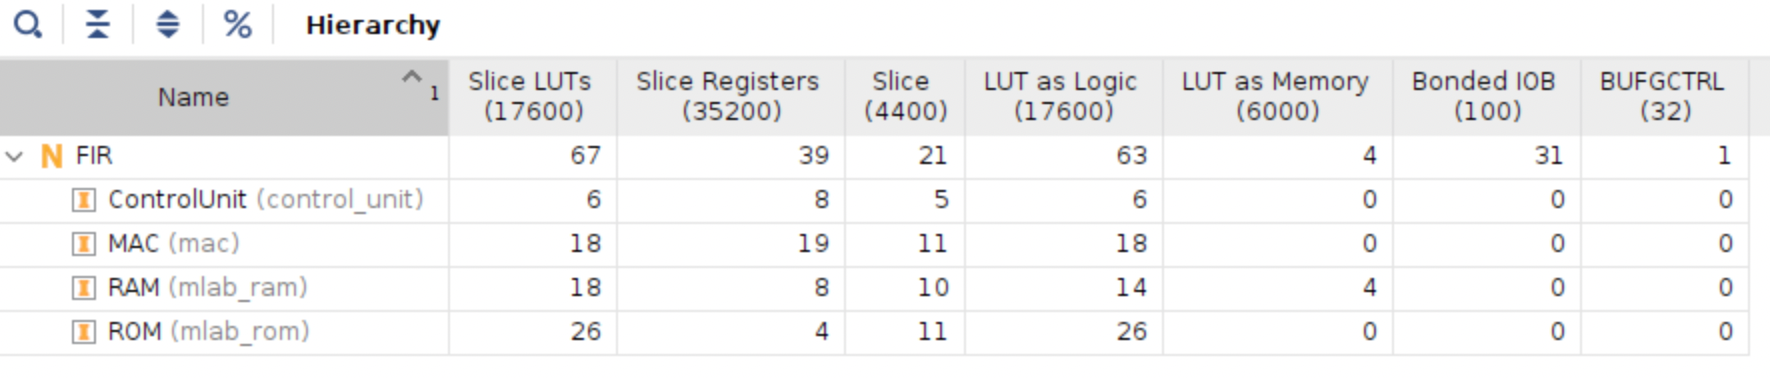
\includegraphics[width=\textwidth]{resource_utilization/resource_utilization.png}
    \caption{Resource Utilization του FIR φίλτρου}
    \label{fig:fir_utilization}
\end{figure}

Από τον πίνακα utilization (Σχήμα \ref{fig:fir_utilization}) προκύπτει η ακόλουθη κατανομή πόρων:

\begin{table}[H]
    \centering
    \begin{tabular}{|l|c|c|c|c|c|}
        \hline
        \textbf{Module} & \textbf{Slice LUTs} & \textbf{Slice Regs} & \textbf{Slices} & \textbf{LUT Logic} & \textbf{LUT Mem} \\
        \hline
        \textbf{FIR (σύνολο)} & 67 & 39 & 21 & 63 & 4 \\
        \hline
        ControlUnit & 6 & 8 & 5 & 6 & 0 \\
        \hline
        MAC & 18 & 19 & 11 & 18 & 0 \\
        \hline
        RAM & 18 & 8 & 10 & 14 & 4 \\
        \hline
        ROM & 26 & 4 & 11 & 26 & 0 \\
        \hline
    \end{tabular}
    \caption{Κατανομή πόρων ανά module}
\end{table}

Παρατηρήσεις:
\begin{itemize}
    \item Η \textbf{ROM} καταλαμβάνει τους περισσότερους LUTs (26), λόγω της αποθήκευσης των συντελεστών σε LUT-as-Logic (distributed ROM).
    \item Η \textbf{MAC} χρησιμοποιεί τους περισσότερους Slice Registers (19), λόγω του 19-bit συσσωρευτή.
    \item Η \textbf{RAM} χρησιμοποιεί 4 LUT-as-Memory για τον υλοποίηση της sliding window μνήμης.
    \item Συνολικά: \textbf{67 Slice LUTs}, \textbf{39 Slice Registers}, \textbf{21 Slices}, \textbf{31 Bonded IOBs}, \textbf{1 BUFGCTRL}.
\end{itemize}

\subsection*{Κατανάλωση Ισχύος (Power)}

\begin{figure}[H]
    \centering
    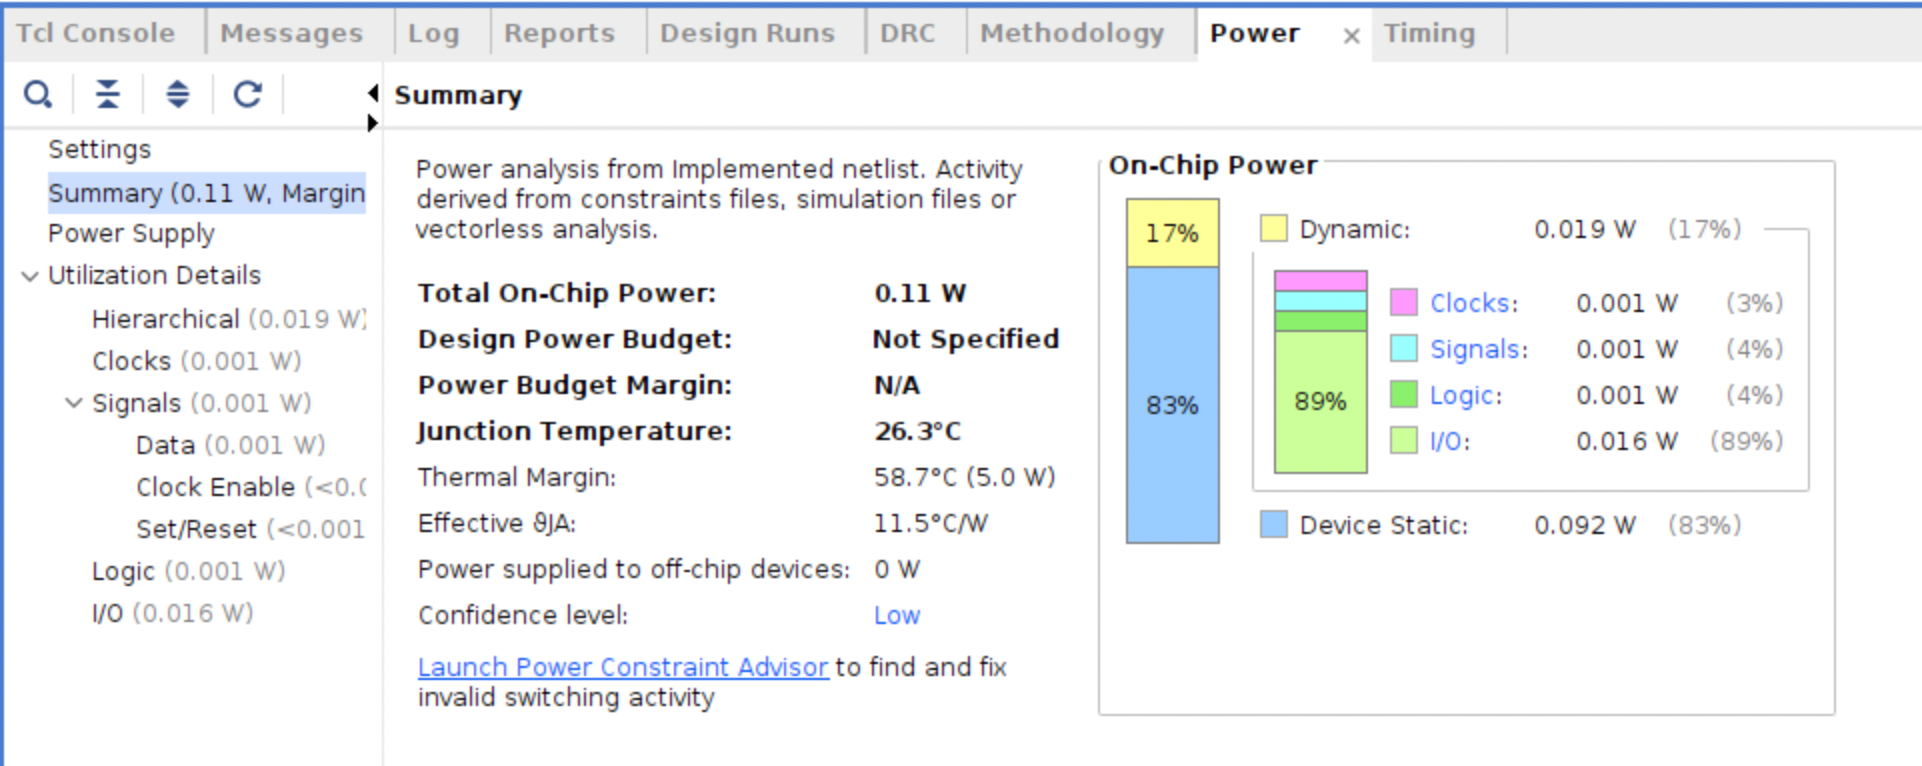
\includegraphics[width=0.85\textwidth]{resource_utilization/power_utilization.png}
    \caption{Power Summary του FIR φίλτρου}
    \label{fig:fir_power}
\end{figure}

Η συνολική κατανάλωση ισχύος είναι \textbf{0.11 W}, εκ των οποίων:
\begin{itemize}
    \item \textbf{Dynamic Power}: 0.019 W (17\%) -- Clocks: 0.001 W, Signals: 0.001 W, Logic: 0.001 W, I/O: 0.016 W.
    \item \textbf{Device Static}: 0.092 W (83\%).
    \item Θερμοκρασία επαφής (Junction): \textbf{26.3°C}, με thermal margin 58.7°C.
\end{itemize}

% ==============================================================================
% SECTION 5: Κρίσιμο Μονοπάτι και Timing
% ==============================================================================
\section*{Κρίσιμο Μονοπάτι και Χρονική Ανάλυση}

\begin{figure}[H]
    \centering
    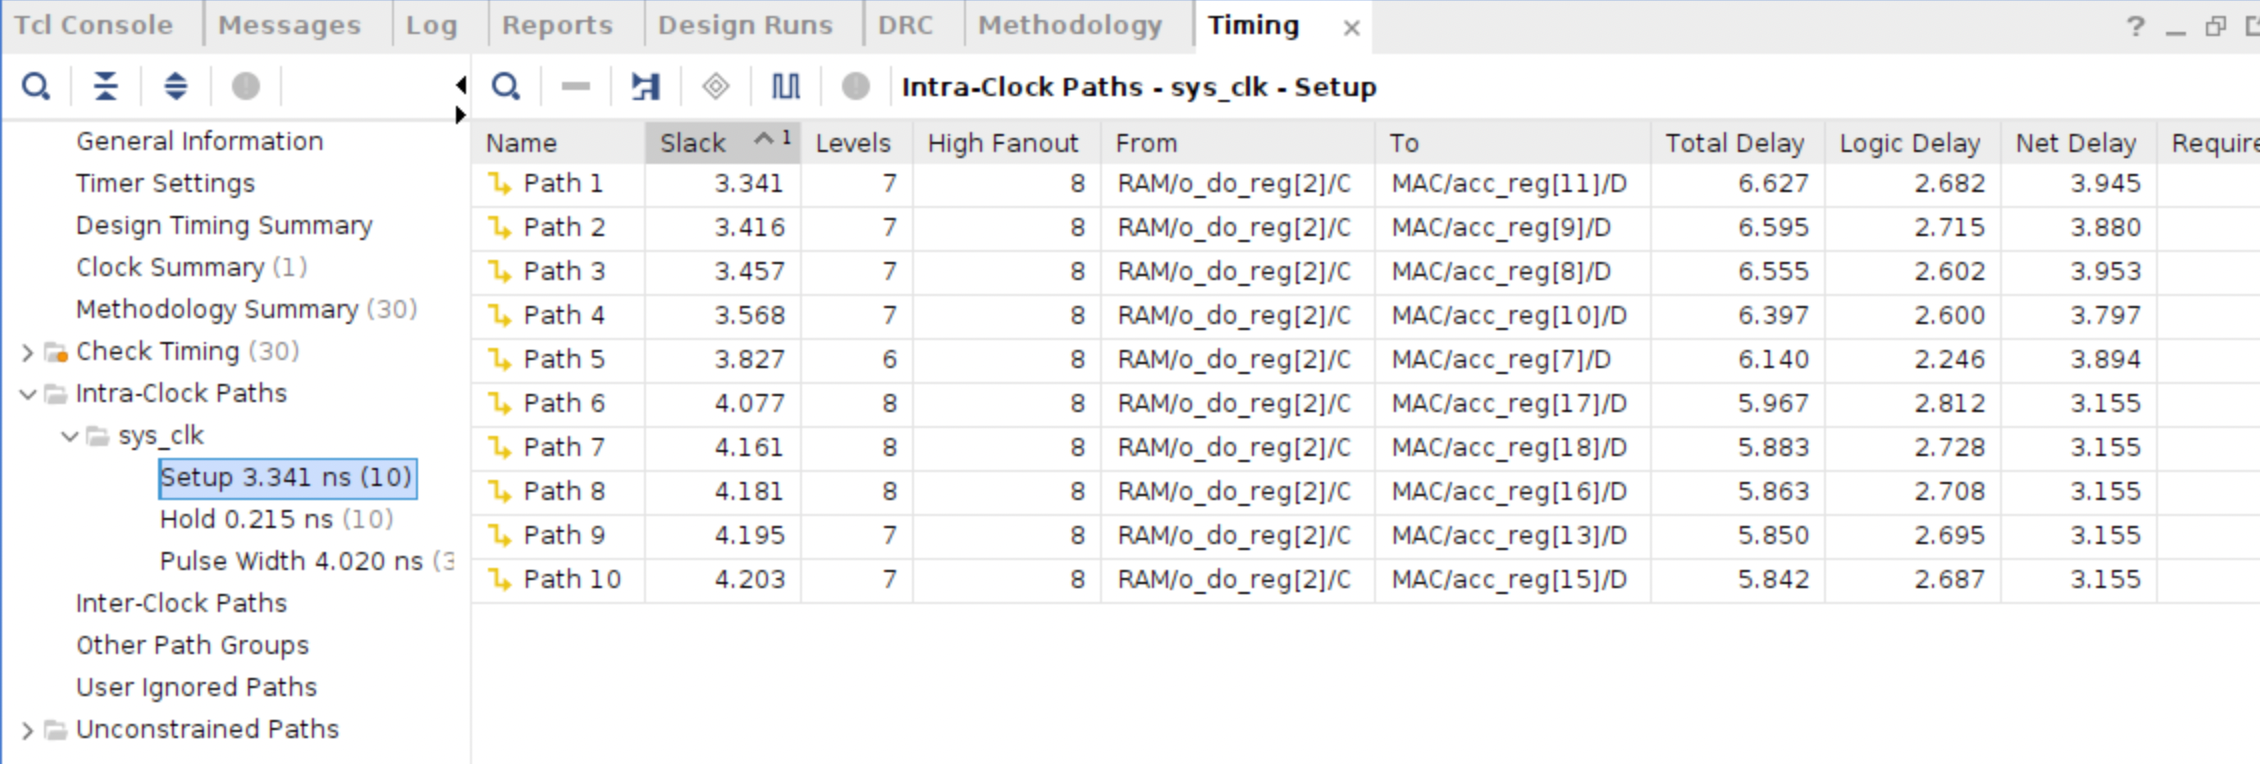
\includegraphics[width=\textwidth]{critical_paths/critical_paths.png}
    \caption{Intra-Clock Paths -- Κρίσιμα μονοπάτια FIR}
    \label{fig:fir_critical}
\end{figure}

\begin{figure}[H]
    \centering
    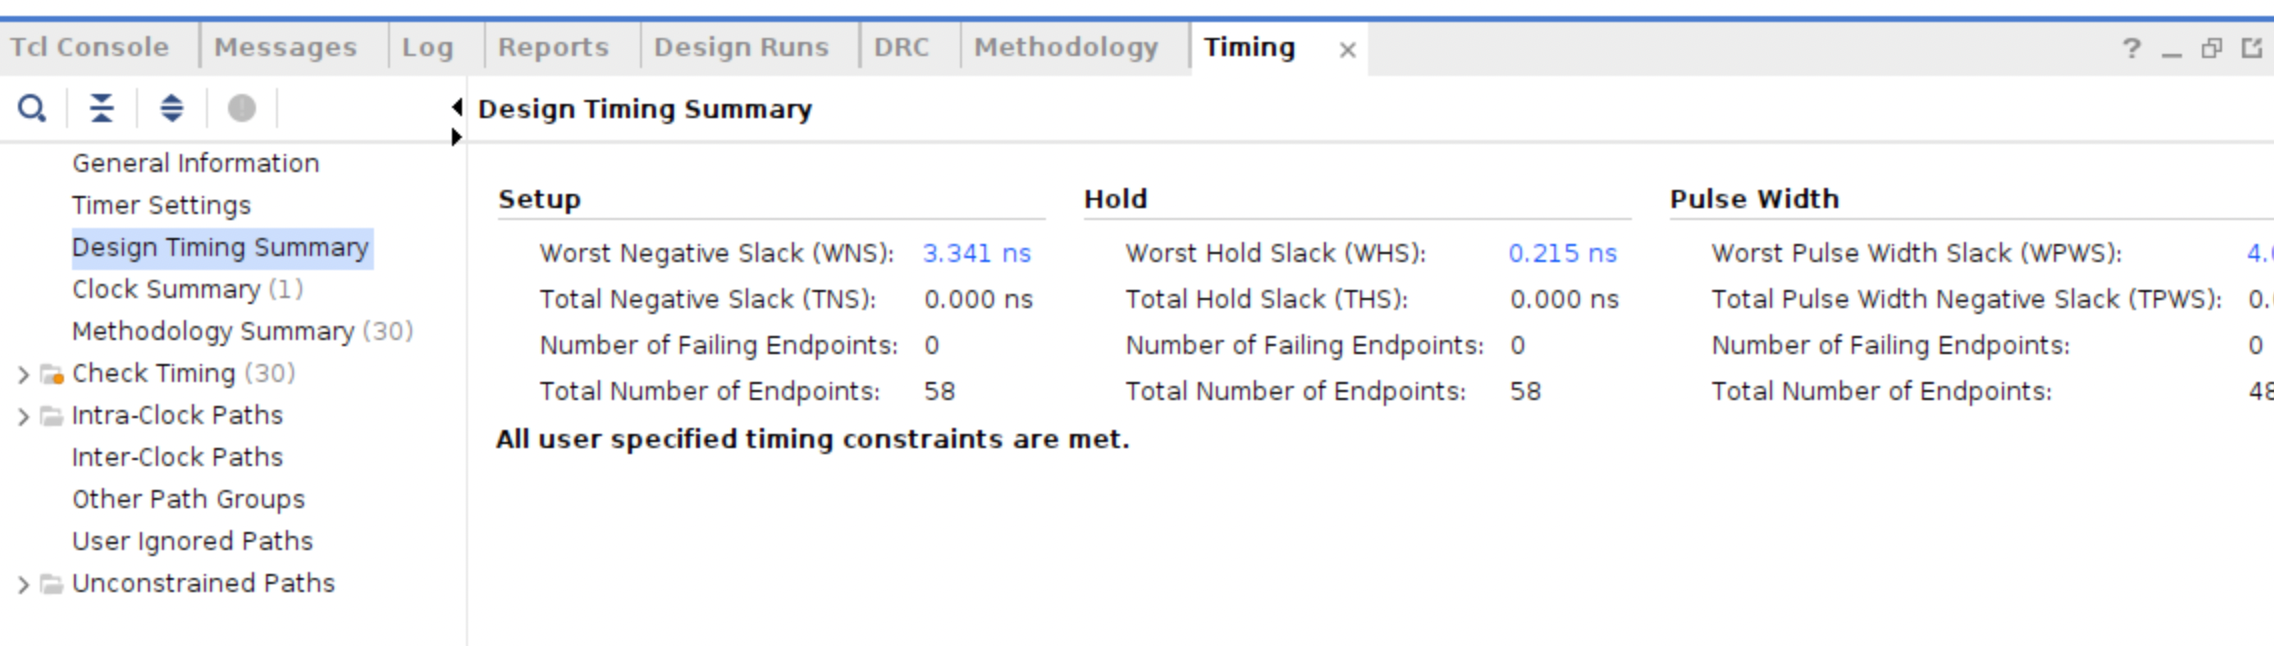
\includegraphics[width=\textwidth]{critical_paths/timing_summary.png}
    \caption{Design Timing Summary του FIR φίλτρου}
    \label{fig:fir_timing}
\end{figure}

Το ρολόι ορίζεται με περίοδο \textbf{8 ns} (125 MHz) μέσω του constraint:

\begin{lstlisting}[language={}]
create_clock -add -name sys_clk_pin -period 8.00 -waveform {0 4}
             [get_ports { i_clk }];
\end{lstlisting}

Από το Design Timing Summary (Σχήμα \ref{fig:fir_timing}) παρατηρούμε:
\begin{itemize}
    \item \textbf{Setup -- WNS = 3.341 ns}: Ικανοποιείται με σημαντικό περιθώριο.
    \item \textbf{Hold -- WHS = 0.215 ns $> 0$}: Δεν υπάρχουν hold violations.
    \item \textbf{Pulse Width -- WPWS = 4.020 ns $> 0$}: Εντός προδιαγραφών.
    \item \textbf{Failing endpoints}: 0 -- πλήρης επιτυχία σε όλα τα 58 endpoints.
\end{itemize}

Το \textbf{κρίσιμο μονοπάτι} (Path 1, Σχήμα \ref{fig:fir_critical}) εκτείνεται από:
\[
    \texttt{RAM/o\_do\_reg[2]/C} \;\longrightarrow\; \texttt{MAC/acc\_reg[11]/D}
\]
με συνολική καθυστέρηση \textbf{6.627 ns} (Logic Delay: 2.682 ns, Net Delay: 3.945 ns) και \textbf{7 επίπεδα λογικής}. Πρόκειται για μονοπάτι register-to-register που διατρέχει τη MAC (πολλαπλασιασμός + πρόσθεση στον accumulator). Το slack του είναι 3.341 ns.

Η μέγιστη συχνότητα λειτουργίας του κυκλώματος είναι:
\[
    f_{\max} = \frac{1}{T_{\text{clk}} - \text{WNS}} = \frac{1}{8\,\text{ns} - 3.341\,\text{ns}} = \frac{1}{4.659\,\text{ns}} \approx \mathbf{214.6\,\text{MHz}}
\]

Το κρίσιμο μονοπάτι διέρχεται από τη RAM (έξοδος καταχωρητή) μέσω του πολλαπλασιαστή/αθροιστή της MAC, γεγονός αναμενόμενο καθώς η MAC εκτελεί τη βαρύτερη αριθμητική πράξη (18-bit accumulate + 8x8 multiply) σε έναν κύκλο ρολογιού.

\end{document}
